%----------------------------------------------------------------------------------------
%	Header stuff that doesn't really matter...
%----------------------------------------------------------------------------------------
\documentclass[paper=letter, fontsize=11pt]{scrartcl}
\usepackage[T1]{fontenc}
\usepackage{fourier}
\usepackage[english]{babel}
\usepackage{amsmath,amsfonts,amsthm}
\usepackage{caption}
\usepackage{sectsty}
\usepackage{graphicx}
\usepackage{float}
\allsectionsfont{\normalfont\sffamily\bfseries}
\usepackage{fancyhdr}
\fancyhead[R]{Phil Crumm 804-005-575 | Connor Proctor 703-999-284}
\fancyfoot[L]{}
\fancyfoot[C]{}
\fancyfoot[R]{\thepage}
\renewcommand{\headrulewidth}{0pt}
\renewcommand{\footrulewidth}{0pt}
\setlength{\headheight}{13.6pt}

%----------------------------------------------------------------------------------------
%	Title area
%----------------------------------------------------------------------------------------

\newcommand{\horrule}[1]{\rule{\linewidth}{#1}}

\title{	
\normalfont \normalsize 
\textsc{University of California, Los Angeles} \\ [25pt]
\horrule{0.5pt} \\[0.4cm]
\Large Computer Science M152A - Digital Design Lab \\
\horrule{2pt} \\[0.5cm]
}

\author{Phillip Crumm \\*804-005-575 \\* Connor Proctor \\* 703-999-284 \\* \\*Lab 2: 4-Bit Serial Adder Implementation}

\date{\normalsize February 4, 2014}
\usepackage[parfill]{parskip}
\begin{document}

\clearpage\maketitle
\thispagestyle{empty}
\pagebreak

%----------------------------------------------------------------------------------------
%	The body
%----------------------------------------------------------------------------------------

\section{Objective}
This laboratory's purpose is to breadboard a 4-bit serial adder using two four-bit shift registers and one bit of a four-bit adder. 

\section{Design}
We utilize an eight-count clock to generate control codes for the addition process. The first four counts (0 to 3) are used to load the bits specified by the selector switches into the shift registers, designated as A and B. The final four counts (4 to 7) are used to conduct the addition. To respect the two-shift-register limitation, we load the output of the adder back into shift register B.

Utilizing an eight-count (three bit) clock to generate control codes simplifies any necessary switching expression greatly. We are able to implement our design using only three individual multiplexer selection bits (one for each bit of the clock).

\section{Implementation}


\begin{figure}[H]
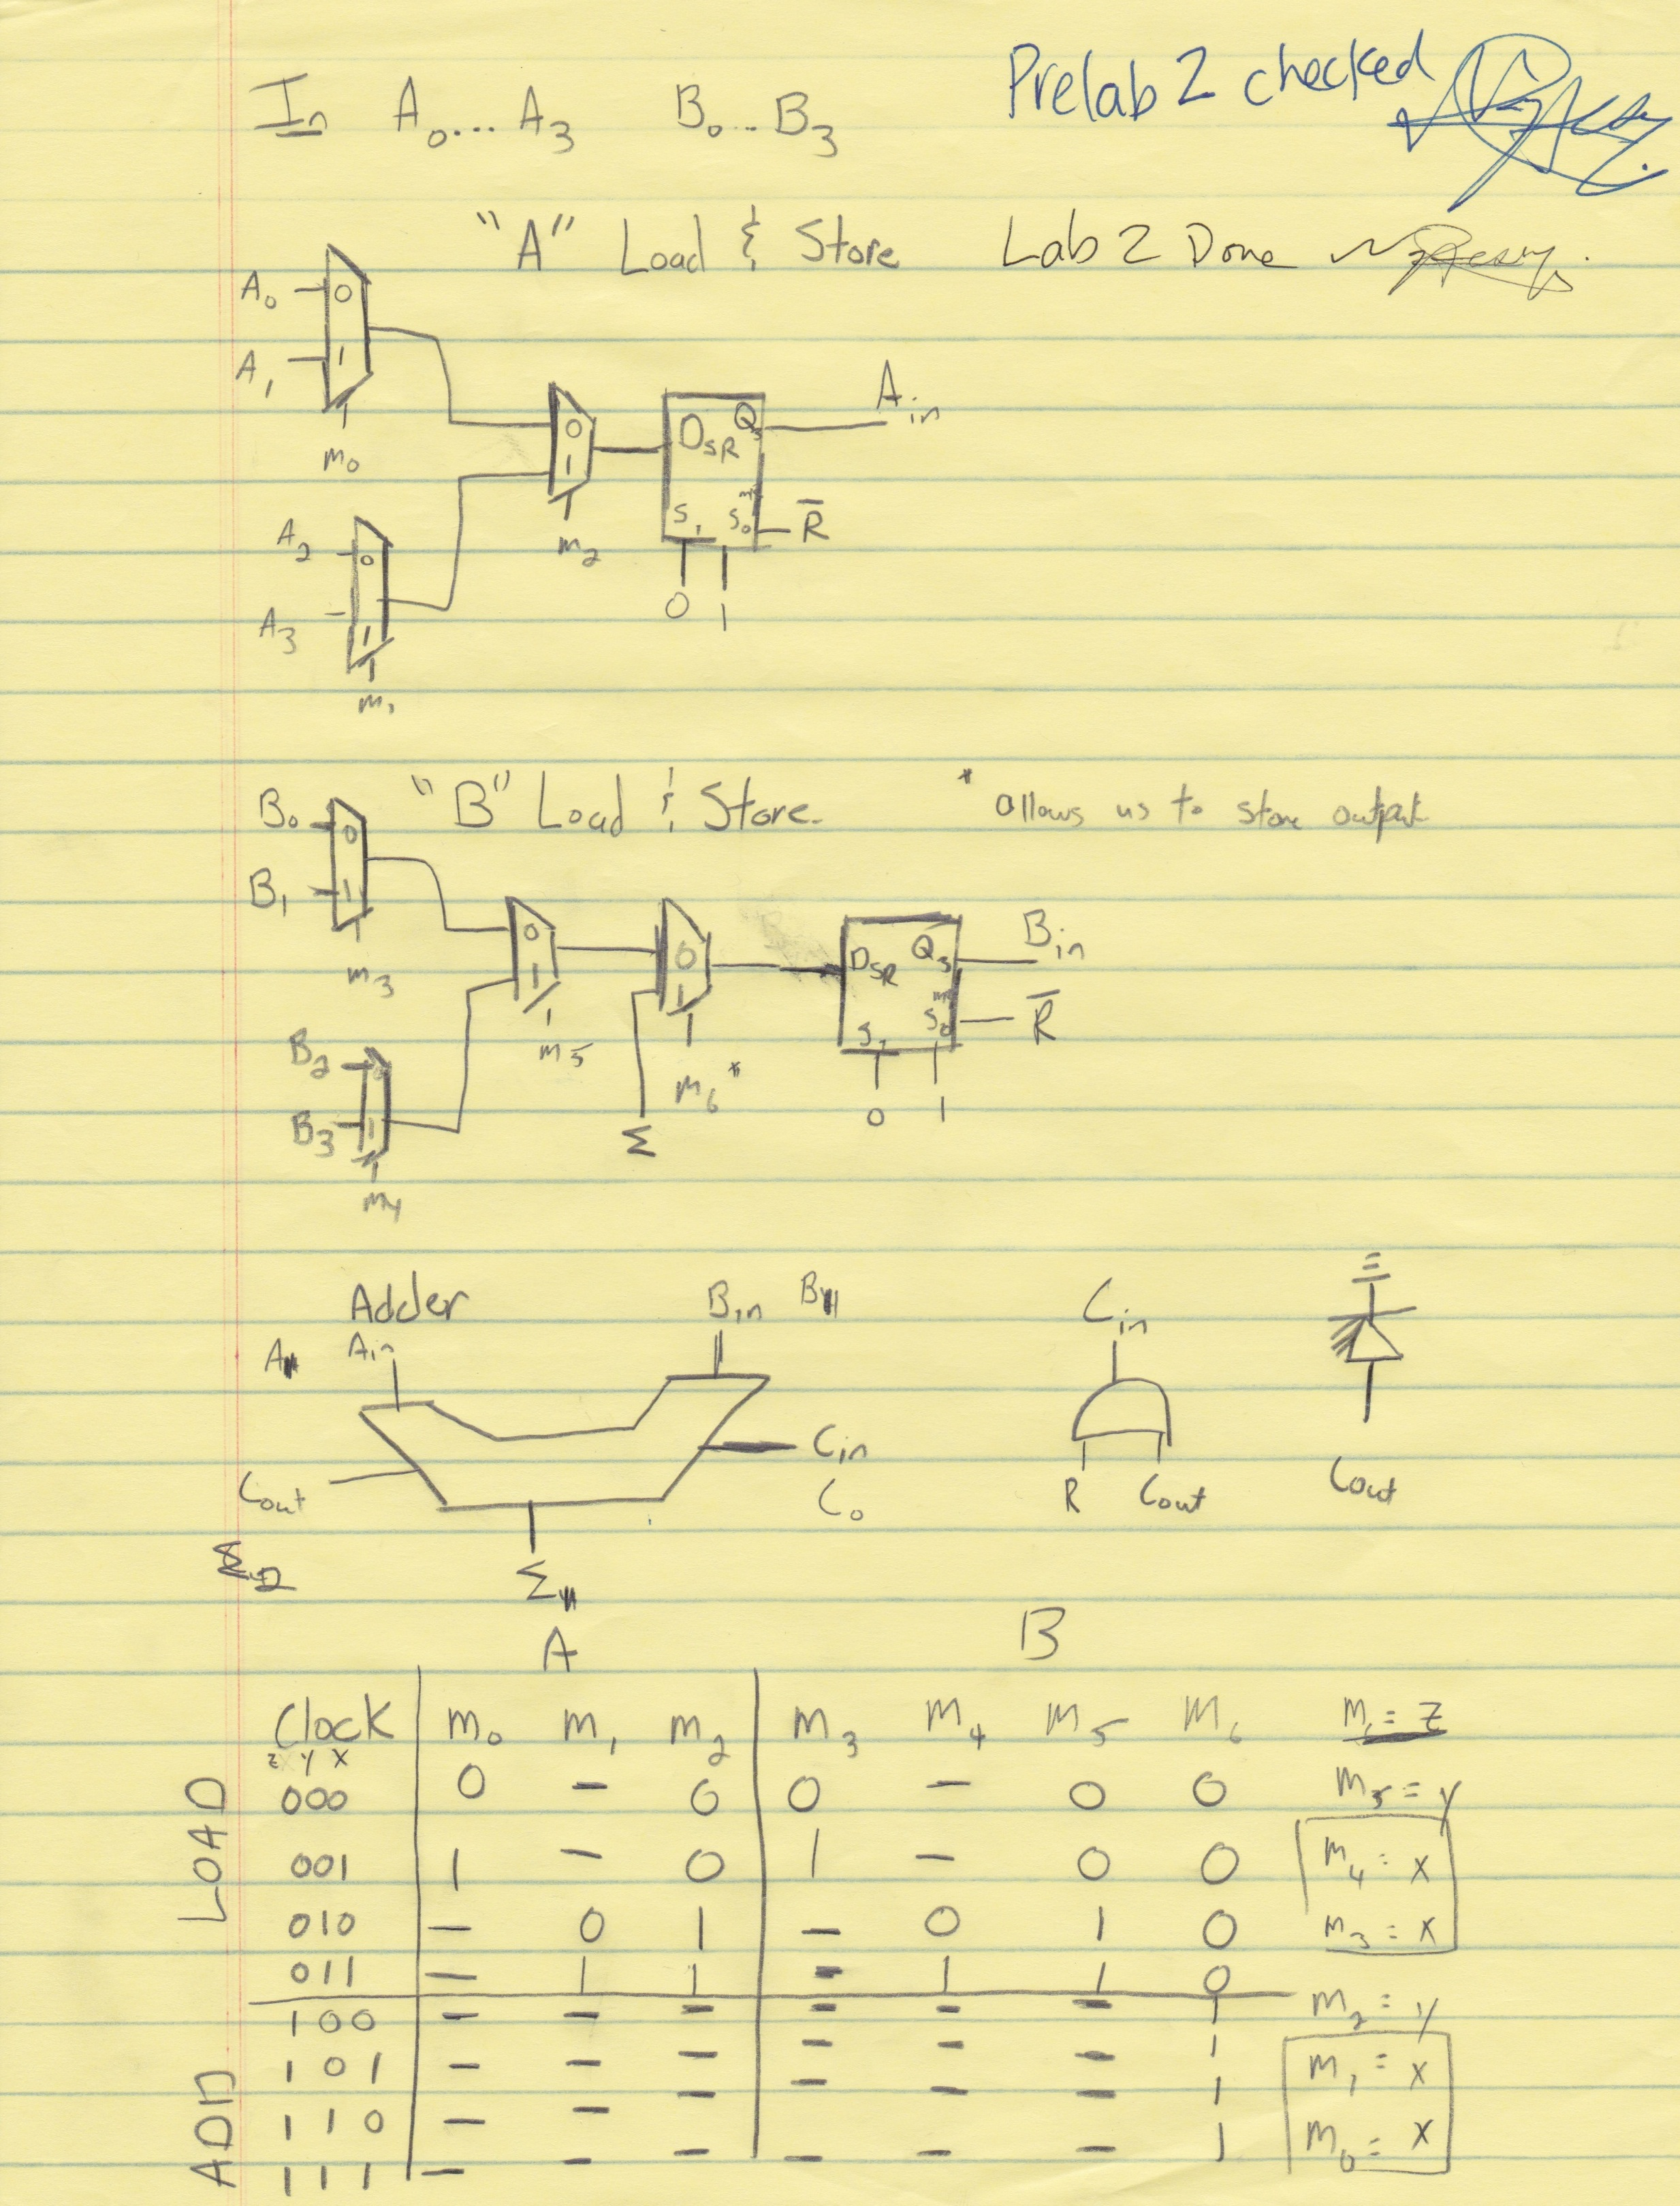
\includegraphics[height=180mm]{prelab2.jpg}
\centering
\caption{Schematic}
\label{overflow}
\end{figure}

We are able to implement our design very simply. To advance the clock and provide reset functionality, we utilize two de-bounced input buttons; the implementation of these buttons is specified in the lab manual and is not duplicated here for conciseness.

From here, the clock is used to control a series of multiplexers. Prior to the first clock iteration (on count 0), we must specify our two desired inputs on the provided switches; again, the exact wiring of these switches is provided in the lab manual and is not duplicated here. On clock cycles 0 through 3, we use a series of multiplexers, each controlled by a clock bit, to load the correct number on the A and B side into the shift register. At the end of cycle 3, each 4-bit number is loaded in its entirety into the 4-bit shift register, with the least significant bit (LSB) of each number held in the rightmost position of the register.

On clock cycles four through eight, we perform an addition and save the result into the leftmost position of register B. The carry-out bit is placed into a D flip-flop, and is loaded back into the adder during the next clock cycle. At the end of this addition, the four bits of the shift register (representing the four bits that are the result of the serial addition) will be available for display on the board's built in LED; this is a trivial connection and is not included in Figure 1 for the sake of brevity.

The fifth bit of the addition may be read from the carry-out D flip flop at the end of the addition. For this display, we utilized an additional diode that we placed directly on the breadboard. This is depicted in Figure 1.

%----------------------------------------------------------------------------------------

\end{document}